
\subsection{\colorbox{red!80}{\parbox{\textwidth}{PT20-FAIL: Awaria serwera powodowana uczciwymi akcjami}}}

\subsubsection{Opis}
Mówiąc żartobliwie, najbezpieczniejsza aplikacja to ta, która na nic nie pozwala. Ważnym elementem poprawiania aplikacji jest upewnienie się, że zachowa ona wszystkie funkcjonalności, co niestety w przypadku badanej wersji wydaje się być niespełnione.

Próba wykonania zamówienia w pełni uczciwy sposób kończyła się awarią aplikacji.
\subsubsection{Warunki wykonania ataku}
Brak. Wystarczy, że użytkownik chce skorzystać z aplikacji do zakupu.

\subsubsection{Szczegóły wykonania}
Próba zamówienia dowolnego produktu działa poprawnie do momentu zakończenia dodawania adresu. Następnie, kiedy dochodzi do etapu wyboru metody przesyłki nie są dostępne żadne opcje, a po przejściu na inne moduły strony są one puste i zaczynają być zwracane błędy 502 Bad Gateway i sklep całkowicie przestaje działać. Jest to oczywiście niedopuszczalne, ponieważ uczciwi użytkownicy (czyli zdecydowana większość) nie mogą dokonać zakupu w aplikacji, która jest sklepem.

Awaria serwera kończyła się restartem połączonym z wyczyszczeniem danych. Nawet bezpośrednio po tym ponowne próby kończyły się równie źle, dlatego nie ma możliwości by to był skutek uboczny testów penetracyjnych.

\begin{figure}[H]
\caption{Brak możliwości wyboru metody(szybkości) dostawy}
\centering
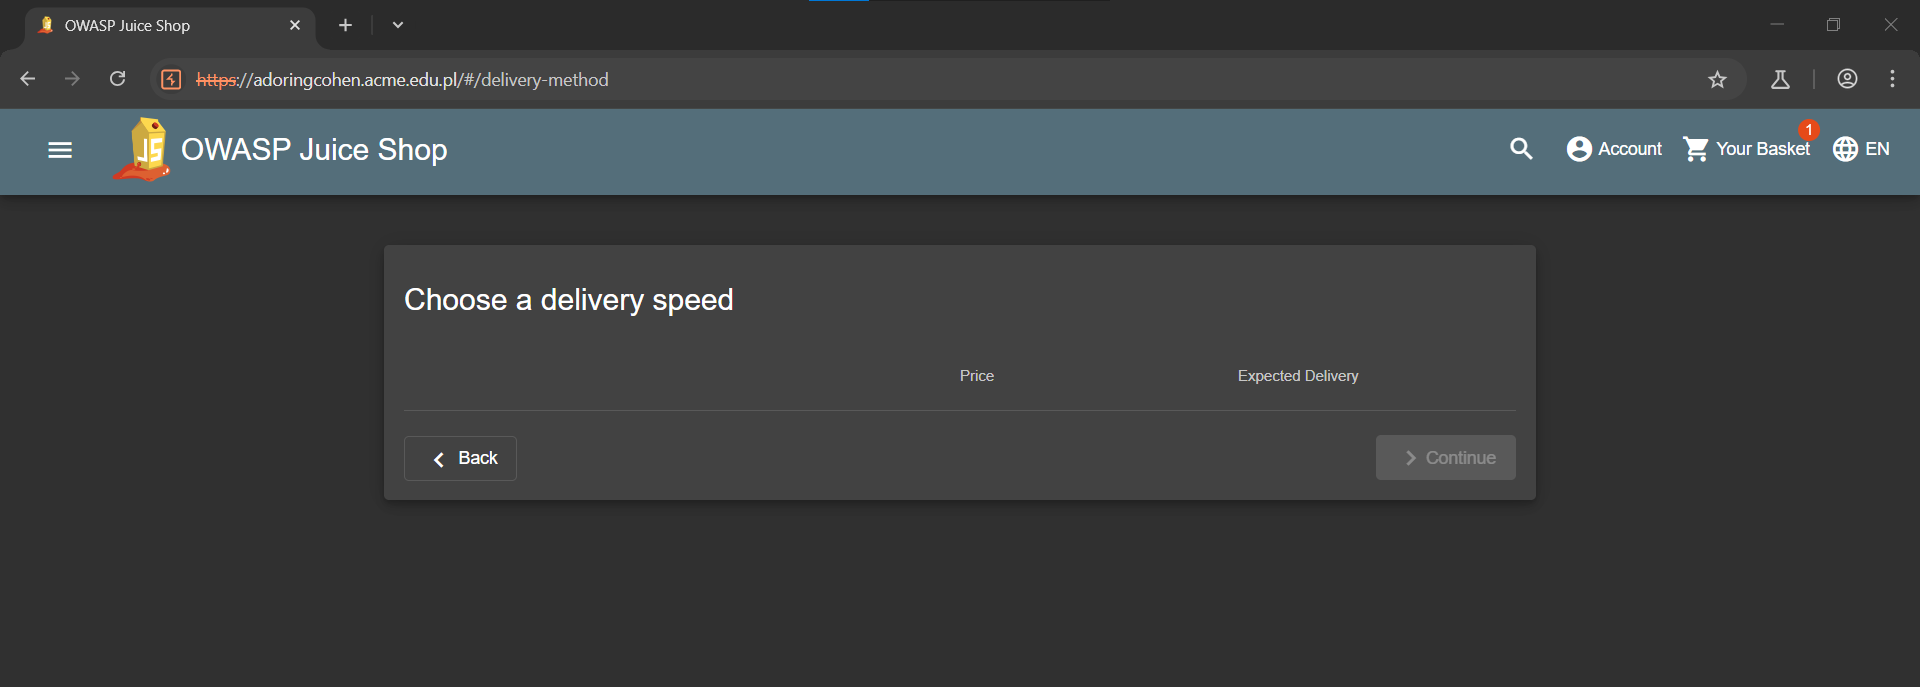
\includegraphics[width=0.8\textwidth]{img/ss1.png}
\end{figure}

\begin{figure}[H]
\caption{Komunikat o awarii aplikacji/serwera będący następstwem próby zamówienia}
\centering
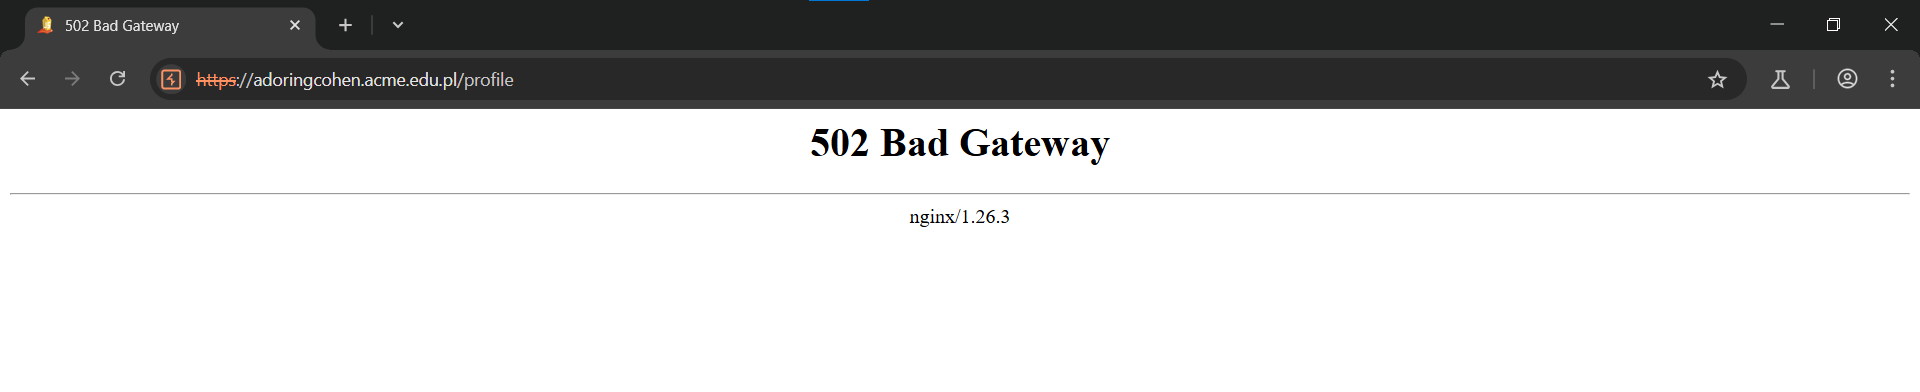
\includegraphics[width=0.8\textwidth]{img/ss2.png}
\end{figure}


\subsubsection{Skutki}

Uczciwy użytkownik może nieumyślnie \textbf{spowodować awarię aplikacji i wyczyszczenie danych}.

\subsubsection{Zalecenia}
Testy jednostkowe. Wprowadzanie zmian powinno być połączone z częstym uruchamianiem testów, które zagwarantują, że żaden moduł nie został przypadkowo uszkodzony.

Ponadto, nawet po awarii dane nie powinny być usuwane. Można to zapewnić przez użycie baz zapisujących dane w trwałych lokalizacjach w systemie plików. 
 

